\begin{document}
We are going to touch on some essential features and metrics that characterize a network.

\section{Sharing}
Sharing is an essential part of networks, as we can reduce the amount of long links needed to connect multiple devices. 
\begin{figure}[!htbp]
    \centering
    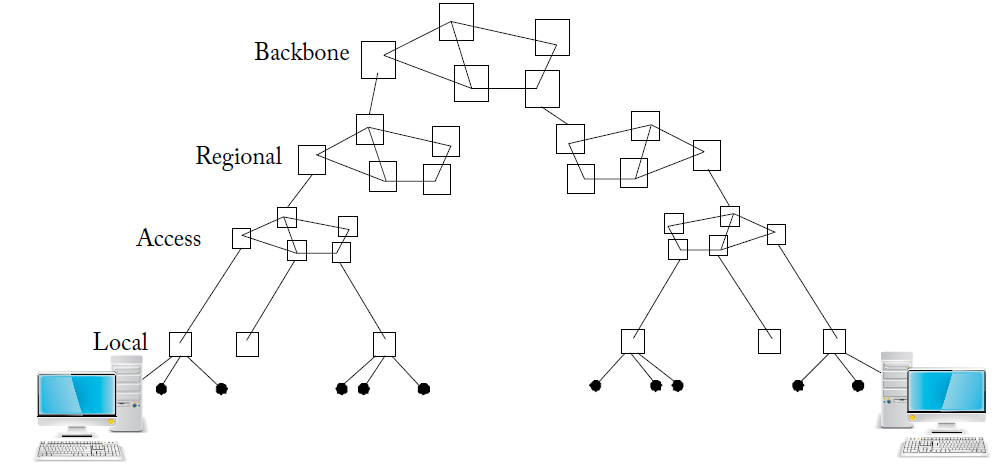
\includegraphics[width=0.75\textwidth]{fig2_1_networkhierarchy}
    \caption{Hierarchy of networks where multiple devices are sharing a local network, multiple local networks are sharing an access networks, and so on}
    \label{fig:Network_Hierarchy}
\end{figure}
\subsubsection*{Multiplexing Gain}
Sharing is possible because devices are not active all of the time. Multiplexing gain measures the benefit of sharing a link between many users and is the amount of active users sharing a link. If $C$ is the link data rate, $M$ is the multiplexing gain, and $C_{user}$ is the data rate seen by the user.
$$ C_{user} = C/M $$
ex. A thousand users are sharing a link, but only ten are active.
$$ C_{user} = C/10 bps$$
\subsubsection*{Link Rate}
Each link is characterized by data rates in bits per second.
ex. Common link rates for cable modem uplink (device to Internet) are 131 Mbps and downlink rate (Internet to device) are 343 Mbps. \\
ex. Links are broadband if its rate exceeds 25 Mbps
downlink and 4 Mbps uplink. If its rate does not exceed that amount it is considered narrowband.
\subsubsection*{Frequency}
Cycles per second (Hz). \\
ex. $V(t) = A sin(2 \pi f_0 t)$, $f_0$ is the frequency
\subsubsection*{Bandwidth}
Measures the width of the range of frequencies on a link.\\
ex. A telephone line can transmit signals over a range of 300 Hz to 1 MHz, so the bandwidth is $$10^6 - 300 = 999700 Hz \approx 1 Mhz$$
\subsubsection*{Signal to Noise Ration (SNR)}
The ratio of the power of the signal at the receiver over the power of the noise at the receiver. Sometimes given in dB, but we would link the ratio. 
$$dB = 10log_{10}(ratio)$$
\subsubsection*{Shannon Capacity}
The larger the bandwidth of a link the faster the link rate. The noisier the channel is, the smaller the SNR, and the more bandwidth needed to reliably transmit the signal. Shannon Capacity quantifies the relationship between the $C$ the maximum reliable link rate, $SNR$ the noise, and $W$ the bandwidth. It is also the theoretical link rate limit that can be achieved. 
 $$C = Wlog_2(1+SNR)$$
\subsubsection*{Delay}
The elapsed time for a packet to traverse between two points. Queuing time is the waiting time for a packet at a node before it can be transmitted. Transmission time refers to the time it takes for a packet to be transmitted over a link at the link rate. Propagation time is the time for the physical signal to get from the starting point to the ending point. Processing time is the time consumed to performing the required operations to process a packet at a node. 
$$Delay_{A\_to\_B} = Q/R + P/R + T_{propagation}$$
$$Delay_{A\_to\_C} = Q/R + 2P/R + T_{processes} + 2T_{propagation}$$

\begin{figure}[!htbp]
    \centering
    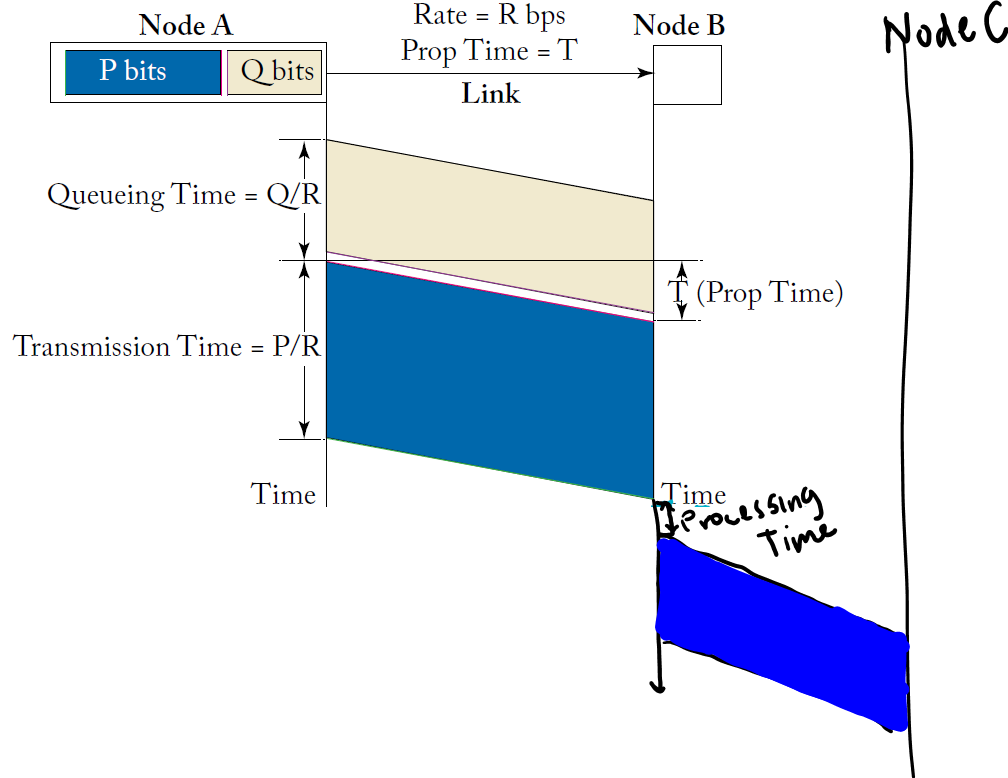
\includegraphics[width=0.5\textwidth]{fig2_2_delay}
    \caption{Delay from Node A to Node B to Node C}
    \label{fig:Delay}
\end{figure}

\subsubsection*{Throughput}
For a particular application, bits per second Not the same as link rate

\end{document}